\renewcommand{\arraystretch}{1.5}
\begin{longtable}{
    |p{4cm}
    |p{8cm}|
}
\caption{Características del sensor seleccionado para la medición de turbidez.}
\label{tab:sensor_turbidez} \\
\hline
\textbf{Característica} 
    & \textbf{Gravity: Analog Turbidity Sensor (SEN0189) \cite{DFRobot_Turbidity_Sensor}} \\ 
\hline
\endfirsthead

\hline
\textbf{Característica} 
    & \textbf{Gravity: Analog Turbidity Sensor (SEN0189) \cite{DFRobot_Turbidity_Sensor}} \\ 
\hline
\endhead

\hline
\multicolumn{2}{r}{\textit{Continúa en la siguiente página}} \\
\endfoot

\hline
\endlastfoot

Tipo de tecnología 
    & Sensor óptico infrarrojo (dispersión de luz) \\ \hline

Rango de medición 
    & 0--1000 NTU \\ \hline

Precisión 
    & Dependiente de la calibración (aproximada) \\ \hline

Tipo de salida 
    & Analógica (0--4.5 V) \\ \hline

Voltaje de operación 
    & 5 V \\ \hline

Compatibilidad con ESP32 
    & Sí (entrada ADC) \\ \hline

Diseñado para monitoreo continuo 
    & No recomendado (sellado básico) \\ \hline

Vida útil de la sonda 
    & 6--12 meses (dependiendo de condiciones ambientales) \\ \hline

Calibración necesaria 
    & Frecuente en ambientes exteriores \\ \hline

Costo aproximado 
    & \$10 USD \\ \hline

Ventajas 
    & Bajo costo, fácil de usar, rápida integración \\ \hline

Desventajas 
    & Precisión limitada, sensibilidad a suciedad y humedad \\ \hline

Imagen
    & \shortstack{\\ 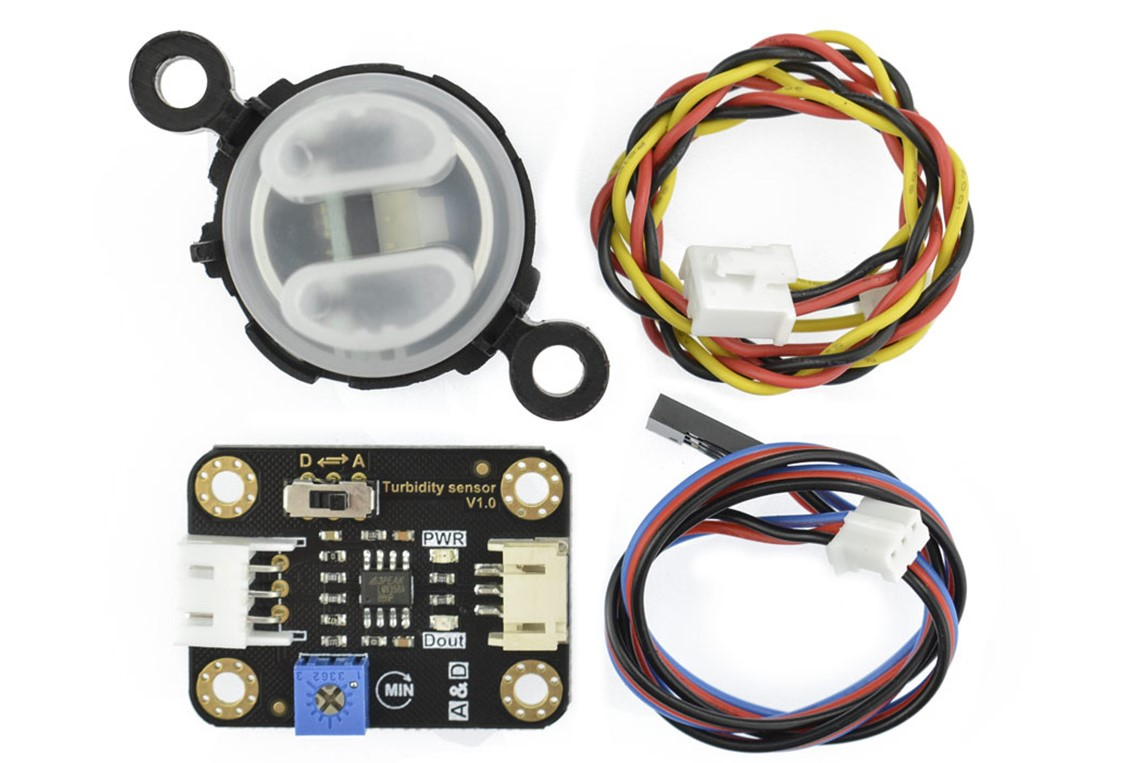
\includegraphics[width=0.7\linewidth]{Documento/Imagenes/Análisis/sensores/turbidez sensor.jpg}} \\ \hline

\end{longtable}
